\section{Test af filtre}
Filtrenes frekvensrespons er målt med et sinus-sweep for et enkelt filter ad gangen. På \autoref{fig:UdregnetKontraPraktiskGain} sammenlignes de fysiske, med de simulerede filtres frekvensrespons. Simuleringerne tager udgangspunkt i ideelle komponentværdier imens de fysiske komponenter kan have små afvigelser, jævnfør \fullref{TilpasningAfFilter}. Kurverne er nærmest identiske, hvilket er yderst tilfredsstillende.
%
\begin{figure}[H]
	\centering
	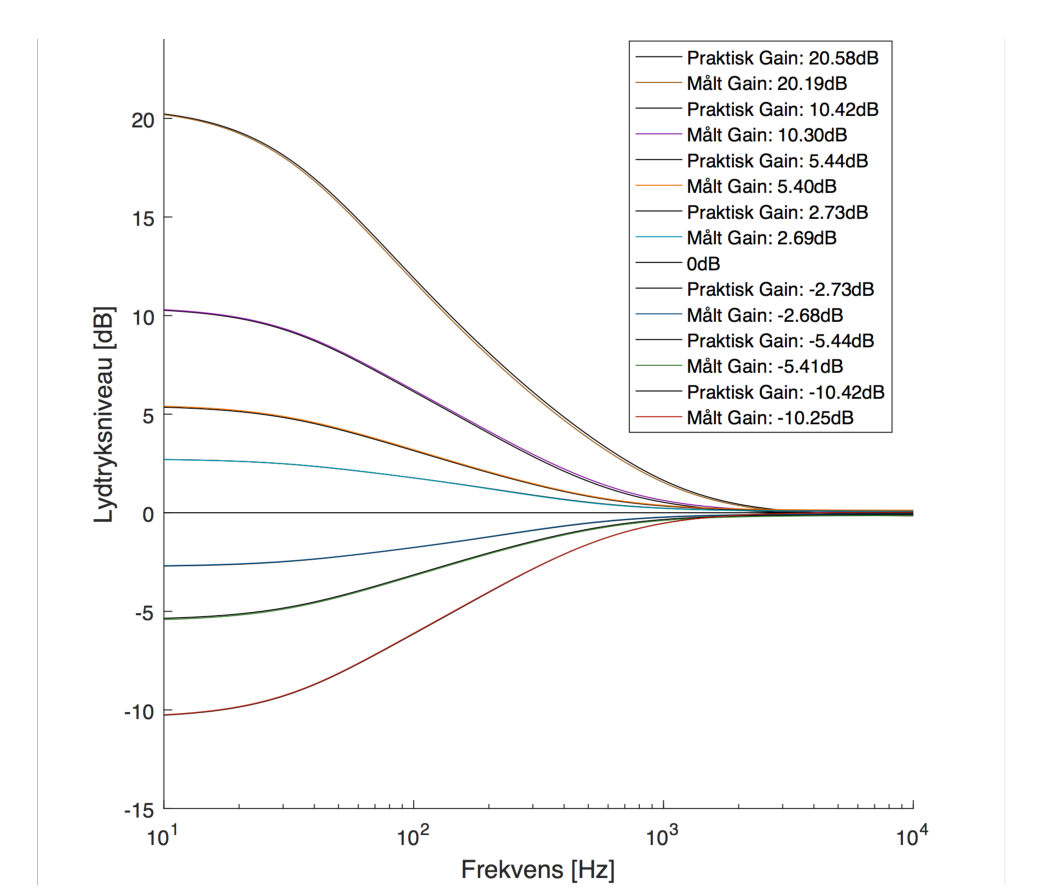
\includegraphics[resolution=300,width=\textwidth]{Figure/DesignAfFilter/PraktiskKontraSweepsSHORT.pdf}
	\caption{Frekvensrespons for simulerede filtre, sammenlignet med målte værdier af fysiske filtre.}
	\label{fig:UdregnetKontraPraktiskGain}
\end{figure}
\noindent
%
THD i de enkelte filtre er særdeles lavt. Dette er meget tilfredsstillende og langt under hvad der var forventet af filtrene. De respektive THD-værdier fremgår af \autoref{tab:THDFiltre}
%
\begin{table}[H]
\centering
\begin{tabular}{|l|l|l|l|l|l|l|l|}
\hline
Filter & 2.62 & 5.24 & 10.48 & 20.96 & -2.62 & -5.24 & -10.48 \\ \hline
THD \% & 0.0025 & 0.0024 & 0.0022 & 0.002 & 0.0027 & 0.0031 & 0.0031 \\ \hline
\end{tabular}
\caption{Sinus-sweep}
\label{tab:THDFiltre}
\end{table}

